\chapter{Análise Bibliográfica sobre O auxílio da indústria dos jogos na evolução do Hardware, por Gabriel Martins de Almeida}

\section{Planejamento do estudo}

Este é um projeto com o propósito de treinar o uso de técnicas de análises bibliométricas para fins de aprendizado. Em resumo, vivemos em um mundo altamente integrado com a tecnologia e embora muitos profissionais, por exemplo, um design gráfico necessita de um processador potente para ter uma boa eficiência no seu trabalho, um usuário comum não necessita do mesmo para o seu ambiente profissional, mas os jogos acabam por levar está necessidade para os clientes usuais. Logo, o lazer relacionado aos jogos aumenta a busca por hardware , então o objetivo é responder as seguintes perguntas.

\begin{itemize}
    \item Quais são os principais usos para o hardware comprado por consumidores comuns?
    \item A evolução do hardware e o aumento dos requisitos de sistemas para jogos estão relacionados?
    \item Com a popularização dos jogos o preço do hardware subiu ou desceu? Quais acontecimentos podem está ligado a esta possível variação?
\end{itemize}

\subsection{Limitações} As limitações estão relacionadas ao tempo, pois é uma atividade introdutória então não foi possível ler os artigos resultantes das buscas e a falta de experiência com a ferramenta pode levar a alguns resultados inesperados.

\section{Coleta de dados} 
Os dados foram coletados na base de dados Web of Science no dia 9 de fevereiro de 2022, acessado por meio do Portal de Periódicos da CAPES

\subsection{Query de Busca}
\begin{verbatim}
A query utilizada para a busca foi:
(game* or  specification or requirements ) 
and 
(advances or computer) 
and 
(hardware or purchase)
\end{verbatim}

\subsection{Explicação para os termos de busca usados}

O primeiro termo utilizado busca informações sobre requisitos e especificações para determinado jogo sendo utilizado o termo game* para buscar dados sobre um jogo e também podendo retornar uma busca para as especificações e requisitos relacionados aos jogadores. O segundo termo busca relacionar o termo a avanços tecnológicos na computação que também está relacionado ao tema da pesquisa, o terceiro tem o proposito de complementar os anteriores tentando buscar informações sobre compras de componentes.

\subsection{Registros recuperados}

A busca retornou 6858 resultados, sendo utilizado uma exportação personalizada passando também como parâmetro as referências citadas, contagem de referências citadas, total de usos e artigos interessantes. Logo, foi feita uma exportação de 5 arquivos de texto sem formatação com um tamanho de 1000 registros e após foi realizada uma concatenação em apenas um arquivo para ser possível passar os 6858 resultados da pesquisa para o biblioshiny.

\section{Análise dos dados}

\subsection{Filtragem de registros}
Após uma filtragem que deu enfoque para os artigos científicos retirando, por exemplo, notas, artigos com acesso antecipado, avaliações de software, etc. foi possível reduzir o número de resultados para 2233.

\subsection{Análise descritiva do dataset}

A descrição das informações principais são:

\begin{description}
    \item [\textit{Timespan}] Os artigos obtidos após a filtragem foram publicados entre o período de 1971 até 2022
    \item [\textit{Sources (Journals, Books, etc)}] Os artigos possuem ao todo 1119 fontes diferentes.
    \item [\textit{Average years from publication}] A média de tempo de publicação dos artigos é de 10.6 anos
    \item [\textit{Average citations per documents}] A média de citações por documentos é 17.33.
    \item [\textit{Average citations per year per doc}] Após o ano de sua publicação, das um dos dos artigos foi citado em média 1.689 vezes por ano.
    \item [\textit{References}] Ao todo, foram feitas 68302 referências por entre os artigos coletados
    \item [\textit{Keywords Plus (ID)}] 0 palavras chaves do tipo ID (Keyword Plus)
    \item [\textit{Author's Keywords (DE)}]  0 palavras chaves escolhidas pelos autores dos artigos

    \item [\textit{Authors}]  são 8105 autores
    \item [\textit{Author Appearances}] 8722
    \item [\textit{Authors of single-authored documents}] Dos 8105 autores, 263 escreveram artigos individualmente
    \item [\textit{Authors of multi-authored documents}] Dos 8105 autores, 263 são autores de artigos escritos em colaboração com outros.
    \item [\textit{Single-authored documents}] São 268 documentos escritos individualmente
    \item [\textit{Documents per Author}] A média de documentos por autor é de 0.276
    \item [\textit{Authors per Document}] A média de autores por documento é de 3.63.
    \item [\textit{Co-Authors per Documents}] As 5749 aparições de autores se distribuem em 3.91 por documento
    \item [\textit{Collaboration Index}] O indíce de colaboração (total de autores em artigos escritos em co-autoria / total de artigos escritos em co-autoria) é de 3.99.
\end{description}


\subsection{Evolução da Produção Científica}

\begin{figure}[ht]
    \centering
    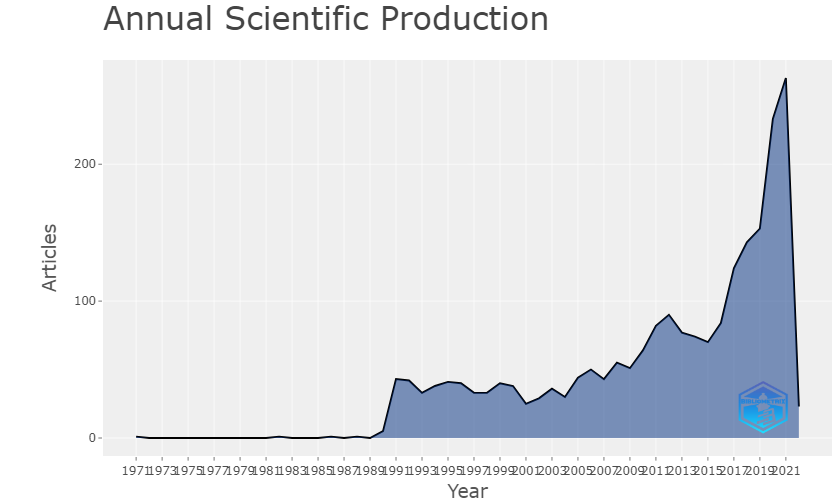
\includegraphics[width=12cm]{experiments/GMalme/AnaliseBibliometrica/ImpactoDeJogosNaTecnologia/Figs/Annual Scientific Production.png}
    \caption{Produção cientifica anual}
    \label{fig:AIJ_produçãoAnual}
\end{figure}

\subsection{Evolução da Produção Científica}

\begin{figure}[ht]
    \centering
    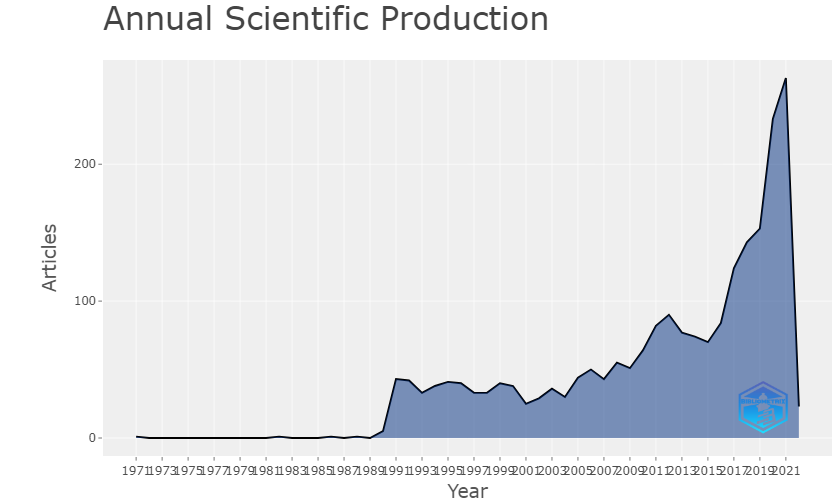
\includegraphics[width=12cm]{experiments/GMalme/AnaliseBibliometrica/ImpactoDeJogosNaTecnologia/Figs/Annual Scientific Production.png}
    \caption{Produção cientifica anual}
    \label{fig:AIJ_produçãoAnual}
\end{figure}

\subsection{Evolução da Produção Científica}

\begin{figure}[ht]
    \centering
    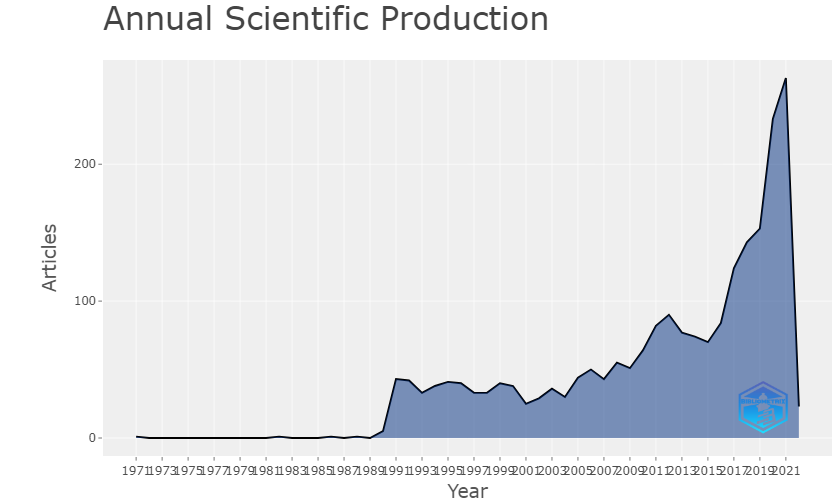
\includegraphics[width=12cm]{experiments/GMalme/AnaliseBibliometrica/ImpactoDeJogosNaTecnologia/Figs/Annual Scientific Production.png}
    \caption{Produção cientifica anual}
    \label{fig:AIJ_produçãoAnual}
\end{figure}

